%=====================================================
% Chapter 0: Topic
%=====================================================

\pagestyle{fancy}
\fancyhead{}
\fancyhead[RE,RO]{\thepage}
\fancyhead[LE]{\slshape \leftmark}
\fancyhead[LO]{\slshape \leftmark}
\fancyfoot{\companyfooter}

\section*{Discussion Question}
 
%<content>%


\begin{quote}

Organisations face a constant battle in choosing between \gls{glos:liquidity} and
\gls{glos:profitability}. A certain degree of both is essential for an entity to survive,
grow and prosper. But managers must constantly choose between the two. Every
investment decision means choosing between liquidity (spending cash) and
increasing future profitability (e.g., by buying new and more efficient
equipment).

   \begin{enumerate}
\item Discuss this ongoing dilemma and its relationship to \gls{glos:accrualsaccounting}. 
\item Explain why profitability is not the same as liquidity and how both are reflected in published financial statements. 
\item Describe how the lack of either could cause an entity to go out of business. 
\item Base your answer upon your reading, further research and your own experience.
   \end{enumerate}
\end{quote}


%</content>% 


\section*{Discussion Question Answer}


%=====================================================
% Include Content and Appendices
%=====================================================

%=====================================================
% Chapter 1: Introduction
% 
% This is not a re-hash of the question but an introduction to your submission
%
% 5% of the word count (50 words)
%=====================================================
% Chapter 1:  5 %  Introduction
% Chapter 2: 30 % Literature Review
% Chapter 3: 40 % Application of the Literature to the Question
% Chapter 4: 20 % Practical Experience
% Chapter 5: 10 % Conclusions
%=====================================================

\section{Introduction}\label{sec:Introduction}
% <content>%



%</content>%






















%=====================================================
% Chapter 2: Literature Review
% 
% Summary of the relevant articles you have located in the library that can 
% be used to help you address the question.
%
% 30% of the word count (300 words)
%=====================================================

\def\hlII{Literature Review}\def\lbII{sec:LiteratureReview}

\mnequals{\doctype}{book}{\chapter{\hlII}}{\section{\hlII}}\label{\lbII}

%<content>%



%</content>%













































































%=====================================================
% Chapter 3: Application of the Literature to the Question
% 
% You use the literature that you have found, together with your own views 
% to formulate your answer
%
% 40% of the word count (400 words)
%=====================================================

\section{Application} \label{sec:Application}
% <content>%

\subsection{Case Study} \label{sec:case_study}

\citeauthor{Vieira:2010ve} applied the findings to the airline industry in the context
of the Lehman crisis (2008) to verify three hypotheses (\citeyear[15]{Vieira:2010ve}):

\begin{enumerate}
  \item \emph{Hypothesis:} ``On the short term  the relationship between liquidity and profitability is negative.'' \label{h1}
  \item \emph{Hypothesis:} ``On the medium term a low liquidity level will derail the upkeep of high 
  profitability, and also a low profitability will derail the upkeep of a high liquidity.'' \label{h2}
  \item \emph{Hypothesis:}``Over the year of 2008, the companies with higher liquidity would be able to
  achieve a better performance.''  \label{h3}
\end{enumerate}

\begin{figure}[htp]
\centerline{\framebox{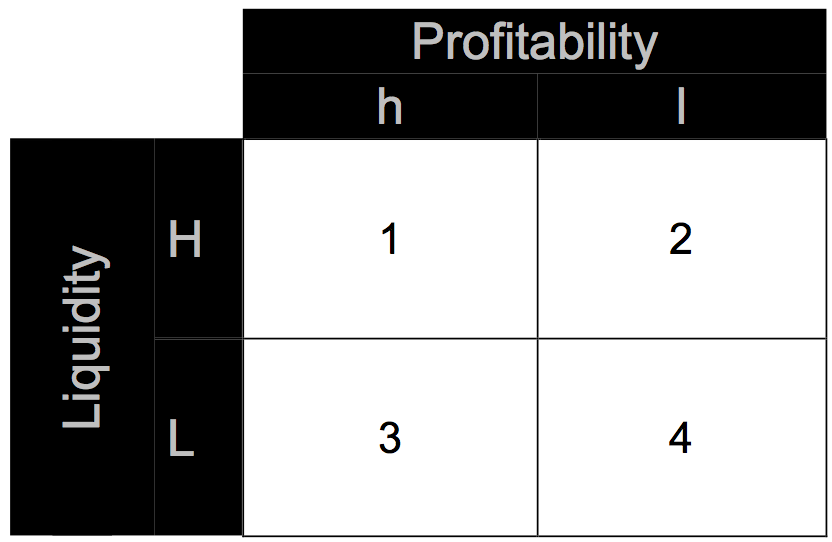
\includegraphics[width=9cm]{fig/plquadrant.jpg}}}
\caption[Liquidity--Profitability--Matrix]{Liquidity--Profitability--Matrix}
\captionsetup{font={footnotesize,it}}
\vspace{-0.3cm}
\caption*{Source: \cite[19]{Vieira:2010ve}}
\label{fig:plquadrant}
\end{figure}

\ni To cluster the companies he observed, \citeauthor{Vieira:2010ve} created a Liquidity--Profitability--Matrix (see
figure \vref{fig:plquadrant}).\endnote{\citeauthor{Vieira:2010ve} clustered the companies using the following rules:

\begin{itemize}
  \item Companies with liquidity ratio $> 1$ go in row \emph{H}, the others in row \emph{L}
  \item Companies with an average \gls{roa} for the observation period higher than the average
  market \gls{roa} went in row \emph{h}, the others in row \emph{l}.
\end{itemize}

\citeauthor{Vieira:2010ve} hypothesized the following behaviors (\citeyear[19]{Vieira:2010ve}):

\begin{itemize}
  \item Companies from quadrant 2 (Hl) would migrate to the quadrants 3 (lH) or 4 (Ll); and companies
  from quadrant 3 (Lh) would migrate to quadrants 2 (Hl) or 4 (Ll) \emph{because the low level of
  one of the indicators would deteriorate the other}.
  \item Companies from quadrants 1 (Hh) or 4 (Ll) would stay there \emph{as their extreme position---either
  good or bad---would lock them in and make it hard to change.}  
\end{itemize}}


\subsection{Results} \label{sec:results}

\subsubsection{Hypothesis 1: Short Term Negative Relationship between Liquidity and Profitability} \label{sec:res_h1}

Interestingly,  hypothesis  \vref{h1} was \emph{clearly rejected}: ``In fact it was
found a significant positive relationship between the indicators.''
(\citeyear[24]{Vieira:2010ve}) This result goes against the literature (see
sections \vref{sec:liquidity_profitability_trade_off} and
\vref{sec:risk_and_returns}), and \citeauthor{Vieira:2010ve} hypothesizes that
the studied industry sector (airlines) might differ significantly from other
sector.\endnote{As an example, this may be due to a high demand on current expenses (fuel, maintenance), hence a
high level of \gls{glos:workingcapital} (see section \vref{sec:cash_gap}) would
be directly related to reducing costs and obtaining higher profits; also, these
companies being rather large, they would be less likely to show a high demand on
liquidity compared to \glspl{glos:sme}---see also \citeauthor{Decman:2012vn} who
note that ``\Glspl{sme} are usually characterized by a high proportion of
current assets to total assets, less liquid, exposed to high volatility of cash
flows and mostly rely on short-term borrowing.'' (\citeyear[692]{Decman:2012vn}).}


\subsubsection{Hypothesis 2: Medium Term, low Liquidity will deteriorate Profitability, and vice versa} \label{sec:res_h2}

Hypothesis \vref{h2} was \emph{confirmed}, yet due to the rejection of hypothesis
\vref{h1}, ``lost part of its meaning:`` \citep[32]{Vieira:2010ve}: An inversion
was not observed, yet a dependency of the medium term relationship on the short
term results.

\subsubsection{Hypothesis 3: Over the year 2008, a higher liquidity helped achieve better performance} \label{sec:res_h3}



The performance indicators observed \emph{strongly confirmed} the hypothesis, as
companies with a higher liquidity had a comparatively better performance in
2008, reinforcing the view that ``the importance of the management of the
working capital increases during hard times.''
(\citeyear[31]{Vieira:2010ve})\endnote{Yet, as hypothesis \vref{h1} was
rejected, this ``lost its original sense, since it was expected that while the
relationship would be negative on the years of prosperity and then become
positive on the years of economic decline.'' (\citeyear[30]{Vieira:2010ve}) }



%</content>%



















%=====================================================
% Chapter 4: Practical Experience
% 
% This is bringing in your experience in relation to the topic, either from 
% your work, or elsewhere. If you don't have any work experience in the 
% topic, you should ask your finance manager at work or CFO for any 
% ideas. If all fails then research on the Internet for relevant examples / 
% experience
%
% 20% of the word count (200 words)
%=====================================================

\def\hlIV{Practical Experience}\def\lbIV{sec:PracticalExperience}

\mnequals{\doctype}{book}{\chapter{\hlIV}}{\section{\hlIV}}\label{\lbIV}

%<content>%



%</content>%















































































% ===================================================== 
% Chapter 5: Conclusions 
% A summary of the key points and a direct response to the question posed  
%
% 5% of the word count (50 words)
% =====================================================

\section{Conclusions} \label{sec:Conclusions}
% <content>%



% </content>%




















%=====================================================
% Static Glossary etc. entries
%=====================================================
%
% Especially interesting if you have acronyms which are only introduced
% within the (later) glossary, hence would not have been used in the text,
% and hence would not appear in the list of acronyms. If you define them
% here, using \glslink{acronymname}{\null}, nothing will be output, yet
% the link will be established, hence the entry will be printed. Likewise,
% you can put here additional things you want to have in the list of acronyms
% (or glossary or symbols, for that matter) even if you do not reference them
% in the text (for whatever reason).
%
%=====================================================

%-----------------------------------------------------
% Samples
%-----------------------------------------------------

% Usage:
%
% \glslink{rosf}{\null}


%-----------------------------------------------------
% Content
%-----------------------------------------------------

%<content>%

\glslink{rosf}{\null}
\glslink{roce}{\null}



%</content>%
























%=====================================================
% Chapter 99: Appendices
%=====================================================

%=====================================================
% Appendix
%=====================================================

\ifthenelse{\equal{\doctype}{book}}{
  \appendix
}{}

%=====================================================
% End Notes
%=====================================================

\phantomsection
\ifthenelse{\equal{\doctype}{book}}{
  \addcontentsline{toc}{chapter}{Notes}
}{
\addcontentsline{toc}{section}{Notes}
}
\pagestyle{fancy}
\fancyhead{}
\fancyhead[RE,RO]{\thepage}
\fancyhead[LE]{\slshape NOTES}
\fancyhead[LO]{\slshape NOTES}
\fancyfoot[C]{}
%\theendnotes \setcounter{endnote}{0}
\label{sec:notes}\printendnotes 
%\setcounter{endnote}{0}
%\clearpage{\pagestyle{empty}\cleardoublepage}
\clearpage




%=====================================================
% Acronyms and Symbols
%=====================================================

\phantomsection
\addcontentsline{toc}{section}{Acronyms and Symbols}
\pagestyle{fancy}
\fancyhead{}
\fancyhead[RE,RO]{\thepage}
\fancyhead[LE]{\slshape ACRONYMS AND SYMBOLS}
\fancyhead[LO]{\slshape ACRONYMS AND SYMBOLS}
\fancyfoot[C]{}
%\printacronym
%\printglossary[type=\acronymtype]
%Print list of acronyms
%\deftranslation[to=German]{Acronyms}{Abk�rzungsverzeichnis}
\label{sec:acronyms}\printglossary[type=\acronymtype,style=long]
%Print list of symbols
\label{sec:symbols}\printglossary[type=symbolslist,style=long]

%\clearpage{\pagestyle{empty}\cleardoublepage}
\clearpage


%=====================================================
% Glossary
%=====================================================

\phantomsection
\addcontentsline{toc}{section}{Glossary}
\pagestyle{fancy}
\fancyhead{}
\fancyhead[RE,RO]{\thepage}
\fancyhead[LE]{\slshape GLOSSARY}
\fancyhead[LO]{\slshape GLOSSARY}
\fancyfoot[C]{}
%\printglossary
%\printglossary[type=main]
\label{sec:glossary}\printglossary[style=altlist,title=Glossary]

%\clearpage{\pagestyle{empty}\cleardoublepage}
\clearpage


%=====================================================
% Index
%=====================================================

% Usage:
% \index{Fourier Series}

%
% Index comes with a plain page style, we hack it here so that we have
% the same pagestyle as everywhere else.
% 
\patchcmd{\theindex}% <cmd>
  {\thispagestyle{plain}}% <search>
  {\pagestyle{indexstyle}}% <replace>
  {}{}%
  \fancypagestyle{indexstyle}{%
\pagestyle{fancy}
\fancyhead{}
\fancyhead[RE,RO]{\thepage}
\fancyhead[LE]{\slshape INDEX}
\fancyhead[LO]{\slshape INDEX}
\fancyfoot[C]{}
 }
\renewcommand{\indexname}{Index}%

\phantomsection
\addcontentsline{toc}{section}{Index}
\label{sec:index}\printindex
%\clearpage{\pagestyle{empty}\cleardoublepage}
\clearpage


%=====================================================
% References
%=====================================================
\phantomsection
\addcontentsline{toc}{section}{References}
\pagestyle{fancy}
\fancyhead{}
\fancyhead[RE,RO]{\thepage}
\fancyhead[LE]{\slshape REFERENCES}
\fancyhead[LO]{\slshape REFERENCES}
\fancyfoot[C]{}
%\begin{thebibliography}{99}
\patchcmd{\bibsetup}{\interlinepenalty=5000}{\interlinepenalty=10000}{}{}
\label{sec:bibliography}\printbibliography
%\end{thebibliography}
%\clearpage{\pagestyle{empty}\cleardoublepage}
%\clearpage


 




